\documentclass[conference]{IEEEtran}
\IEEEoverridecommandlockouts

\usepackage{cite}
\usepackage{amsmath,amssymb}
\usepackage{graphicx}
\usepackage{booktabs}
\usepackage{multirow}
\usepackage{xcolor}
\usepackage{url}

\newcommand{\uS}{\,$\mu$S}
\newcommand{\todo}[1]{\textcolor{red}{[#1]}}

\begin{document}

\title{Sympathetic Arousal During Emotional Films from Skin Conductance}

\author{\IEEEauthorblockN{Eleftherios Komvopoulos and Piyush More}
\IEEEauthorblockA{Tandon School of Engineering, New York University, Brooklyn, NY, USA\\
\{ek4538, pm4081\}@nyu.edu\\
Course project, BE-GY 9603 / ECE-GY 9153, Neural and Physiological Signal Processing}}

\maketitle

\begin{abstract}
Skin conductance reflects sudomotor nerve activity, a branch of the sympathetic nervous system,
but each burst of activity is blurred into a slow response that overlaps with its neighbours. We
recover the bursts with our own implementation of the sparse deconvolution of Amin and Faghih
(2021), which reproduces the published solver's output while exposing every setting, and we tune
it on synthetic sessions built from the participants themselves: each copies one participant's
timeline, responses, tonic level and noise, with a known pulse train and a response shape drawn
within physiological limits. Applied to 50 participants of the POPANE dataset (Study 6) who
watched neutral, positive, negative or mixed films, the frozen solver recovers pulses of at least
0.05\uS{} with F1 0.96 (recall 0.98, precision 0.96) on 50 unseen test sessions, and all pulses
down to 0.02\uS{} with F1 0.82; the re-synthesis test used in the literature gives 0.96 and 0.86.
On the real recordings, the solver counts isolated responses as it does where the truth is known,
apart from about 16\% extra small pulses on response rises, and each participant's pulse rate
tracks their visible responding (rank correlation 0.73). Slow responses remain the hard case:
their decays come out 37\% short, because during dense slow responding the true tonic level is
never visible. \todo{Stage 2: arousal-state estimation and the tests of H1--H6, to be added.}
\end{abstract}

\begin{IEEEkeywords}
Electrodermal activity, skin conductance, sparse deconvolution, sudomotor nerve activity,
sympathetic arousal, emotion, synthetic validation.
\end{IEEEkeywords}

%=====================================================================
\section{Introduction}

Skin conductance (SC) rises when sudomotor nerves, a branch of the sympathetic nervous system,
trigger sweat secretion, which makes it a common window on sympathetic arousal
\cite{boucsein2012}. The signal combines a slowly varying tonic level with phasic skin
conductance responses (SCRs). Each SCR peaks one to three seconds after it starts and recovers
over several seconds, so responses that follow each other closely overlap. Deconvolution methods
therefore model the phasic part as a sparse train of sudomotor bursts filtered by a response
kernel, and estimate the bursts directly
\cite{benedek2010dda,benedek2010cda,greco2016,amin2021}. Amin and Faghih \cite{amin2021} estimate
the bursts, the kernel's rise and decay time constants and a B-spline tonic jointly, with the
sparsity chosen by generalized cross-validation (GCV) and Gaussian priors on the time constants.

Two obstacles appeared when we applied this approach to an emotion dataset. First, the published
solver is distributed in encrypted form, and in our tests its time constants never left their
prior: when the true response shape differed from the prior, part of each response leaked into
the tonic. Second, these methods are often validated by re-synthesis: the method's output on real
data is rebuilt, noise is added, and the result is deconvolved again \cite{amin2021}. That test is
circular, because pulses the method missed are absent from the truth and its response model is
exact by construction.

This paper reports how we addressed both, and what the resulting pipeline finds on 50
participants who watched emotional films. Our contributions are:
\begin{itemize}
\item an open re-implementation of \cite{amin2021} that reproduces the published solver's output
but exposes every setting (Section~\ref{sec:model});
\item a participant-matched synthetic generator that copies each participant's timeline,
responses, tonic and noise while drawing the response shape at random within physiological
limits, giving a realistic but non-circular ground truth (Section~\ref{sec:synth});
\item tuning in rounds that each change one setting, followed by a single evaluation on unseen
sessions, the re-synthesis test, and model-free checks on the real recordings
(Sections~\ref{sec:tuning} and~\ref{sec:results});
\item \todo{stage 2: estimation of a continuous arousal state from the pulses, and the tests of
the hypotheses below.}
\end{itemize}

The project's hypotheses, stated in the proposal, are: H1, films raise arousal above the resting
baseline; H2, emotional films raise it more than neutral ones; H3 (primary), arousal reflects
intensity alone, so negative and positive films both exceed neutral but do not differ from each
other; H4 (the competing alternative), negative exceeds positive within the same person, in the
mixed group; H5, emotions within a valence do not separate; H6, the decoded state tracks the
participant's own affect rating.

%=====================================================================
\section{Data}

\subsection{Recordings and Protocol}
We use Study~6 of the POPANE dataset \cite{behnke2022}, in which the SC of 187 participants was
recorded at 1000\,Hz with a block code on every sample. After a five-minute resting baseline and
an unlabelled transition (median 150\,s, range 96--338\,s in our sample), each participant
watched 12 minutes of film clips (six clips of 2 minutes), assigned at random to one of four
conditions: neutral, positive, negative, or mixed (in our data, 6 minutes negative and 6 minutes
positive). An ultimatum game followed, which we exclude: the analysed segment runs from the first
baseline sample to the last film sample. Valence was rated continuously on a 1--10 slider.

\subsection{Participant Selection}
Selection used only model-free measures of the baseline, because film-period responding is the
outcome of H1--H3, and was fixed before the selected participants were deconvolved.
Stage~1, a quality screen set before the proposal (the dataset's EDA flag, electrode noise,
missing data, near-flat recordings and non-responders), kept 119 of 187 participants. Stage~2
required a median baseline SCR of at least 0.05\uS: below it most responses lie in
0.02--0.05\uS, where an early synthetic test recovered 58\% of pulses at 65\% precision against
98\% and 96\% above, and 0.05\uS{} is the top of the usual 0.01--0.05\uS{} minimum-response range
\cite{boucsein2012}. It excluded 22 participants (10 negative, 5 neutral, 4 positive, 3 mixed).
Stage~3 drew 20 neutral, 10 positive, 10 negative and 10 mixed participants at random, with a
fixed seed, from the 97 who passed. The four groups did not differ at baseline in SC level, SCR
rate, SCR size or noise (Kruskal--Wallis, all $p > 0.12$).

%=====================================================================
\section{Methods}

\subsection{Model and Solver}\label{sec:model}
Within each analysis window, the phasic SC $y_p$ follows a second-order model driven by the
sudomotor input $u$ \cite{amin2021},
\begin{equation}
\tau_r\tau_d\,\ddot y_p + (\tau_r+\tau_d)\,\dot y_p + y_p = u ,
\end{equation}
so a window of the signal is written
\begin{equation}
\mathbf{y} = a\,\mathbf{y}_0 + \mathbf{B}(\boldsymbol{\tau})\,\mathbf{u} + \mathbf{C}\mathbf{q}
+ \boldsymbol{\nu},
\end{equation}
where $a\,\mathbf{y}_0$ is the decay of the phasic level at the window's start,
$\mathbf{B}(\boldsymbol{\tau})$ maps impulses to responses, the columns of $\mathbf{C}$ are cubic
B-splines with knots every 14\,s (the tonic $\mathbf{C}\mathbf{q}$), and $\boldsymbol{\nu}$ is
noise. The estimate minimizes
\begin{multline}
\tfrac12\bigl\|\mathbf{y}-a\mathbf{y}_0-\mathbf{B}\mathbf{u}-\mathbf{C}\mathbf{q}\bigr\|_2^2
+\lambda_1\|\mathbf{q}\|_2^2+\lambda_2\|\mathbf{u}\|_p^p \\
+\sum_{i\in\{r,d\}}\frac{\lambda_3}{2\sigma_i^2}(\tau_i-\mu_i)^2
\end{multline}
subject to $\mathbf{u}\ge 0$, $\mathbf{C}\mathbf{q}\le\mathbf{y}$, $0\le y_0\le y_1$,
$0.1\le\tau_r\le 2$\,s, $1.5\le\tau_d\le 14$\,s and $\tau_d\ge 1.1\,\tau_r$, with $p=0.5$,
$\lambda_3=2\cdot10^{-4}$ and the prior means and standard deviations of \cite{amin2021}
($\mu_r=0.65$, $\mu_d=2.77$, $\sigma_r=0.21$, $\sigma_d=0.52$\,s).

The problem is solved by block coordinate descent in two phases \cite{amin2021}. In phase~1
(30 iterations), the impulses are updated by FOCUSS+ \cite{gorodnitsky1997}, a reweighted
minimum-norm iteration
$\mathbf{u}\leftarrow\mathbf{P}\mathbf{B}^{\top}(\mathbf{B}\mathbf{P}\mathbf{B}^{\top}
+\lambda_2\mathbf{I})^{-1}\mathbf{r}$ on the current residual $\mathbf{r}$, with
$\mathbf{P}=\mathrm{diag}(|\mathbf{u}|^{2-p})$ and negative entries set to zero, which drives
small impulses to exactly zero. In this phase $\lambda_1=0$ and
$\lambda_2=(1-\|\mathbf{r}-\mathbf{B}\mathbf{u}\|/\|\mathbf{r}\|)\,\lambda_{\max}$ grows as the
fit improves, up to a cap $\lambda_{\max}$ that the paper does not give; impulses closer than 1\,s are pruned to the largest, and at most
the number of SCR peaks plus 20 are kept. Then $\boldsymbol{\tau}$ and $\mathbf{y}_0$ are updated
by an interior-point method, and $\mathbf{q}$ by least squares under the tonic constraint.
Phase~2 repeats the cycle until nothing changes, with GCV-FOCUSS+: the same update, but with
$\lambda_2$ chosen at every iteration by generalized cross-validation \cite{golub1979} below a
fixed cap and impulses whose response would peak below 0.02\uS{} removed; $\lambda_1$ is also
chosen by GCV, below its own cap.
Windows are 200\,s long and start every 100\,s. Each is solved from 8 random starts; the converged
start with the lowest residual whose $\tau_r$ lies off its bounds is kept, and the middle halves
of the windows are joined. Each impulse's height in $\mu$S is its amplitude times the peak of its
window's response.

Rebuilding the published solver's phasic output from its own saved time constants and impulses
with our matrices gave $R^2=1.0000$ (gain 1.000; impulses offset by two samples, an indexing
difference), and its tonic with our basis $R^2\ge 0.997$: our implementation is the same model,
with every setting under our control. Table~\ref{tab:changes} lists where our settings differ from
the paper.

\begin{table}[t]
\centering
\caption{Settings That Differ from Amin and Faghih \cite{amin2021}}
\label{tab:changes}
\footnotesize
\setlength{\tabcolsep}{3pt}
\begin{tabular}{@{}lllp{2.3cm}@{}}
\toprule
Setting & Paper & Ours & Source \\
\midrule
Low-pass / signal rate & 0.5\,Hz / 2\,Hz & 1\,Hz / 4\,Hz & Tuning round 3 \\
$\tau_r$, $\tau_d$ upper bounds & 1.5, 6\,s & 2, 14\,s & Physiological SCR ranges \\
$\tau_d \ge 1.1\,\tau_r$ & -- & added & Keeps the kernel defined \\
Input model & impulse & zero-order hold & Matches the published solver \\
Knot spacing & 6\,s & 14\,s & Rounds 1, 5, 8 \\
Prior weight $\lambda_3$ & 0.1 & $2\cdot10^{-4}$ & Rounds 1, 4; doubled at 4\,Hz \\
Sparsity exponent $p$ & open & 0.5 & Code of \cite{faghih2014} \\
Phase-1 cap $\lambda_{\max}$ on $\lambda_2$ & -- & $2\cdot10^{-3}$ & Round 2; doubled at 4\,Hz \\
GCV caps on $\lambda_2$, $\lambda_1$ & $10^{-4}$ & $2\cdot10^{-4}$ & Doubled at 4\,Hz \\
Impulse cutoff & 3 (in $u$) & 0.02\uS{} height & Same meaning at any $\tau$ \\
Scaling of $\mathbf{y}$ & -- & none ($\mu$S) & Round 6 \\
\bottomrule
\end{tabular}
\end{table}

\subsection{Preprocessing}\label{sec:prep}
All steps run at the recording's 1000\,Hz rate, with a single down-sampling last: gaps are filled
by linear interpolation; jumps (prominence 0.1\uS{} in the 10\,ms change) are replaced over
0.5\,s by a cubic spline through 0.1\,s means; a zero-delay FIR low-pass (Hamming window, 6.4\,s)
at 1\,Hz follows; the signal is cut to the analysed segment, after the filter so its edges fall
outside, down-sampled to 4\,Hz, and shifted by a constant only if it falls below zero. The
paper's 0.5\,Hz filter at 2\,Hz smeared each response by about a second, which the fit read as a
slower rise; at 1\,Hz and 4\,Hz the 2\,Hz Nyquist limit leaves room for the filter's roll-off, and
F1 rose from 0.81 to 0.85 (round 3).

\subsection{Participant-Matched Synthetic Ground Truth}\label{sec:synth}
Each synthetic session copies one of the 50 participants, with nothing fitted across
participants: their timeline; their tonic level, taken as a 60\,s lower envelope of their
recording; their own counted SCRs, reused film by film at random times, so each film keeps its
own response rate and sizes; and their noise, as slow fluctuations and white noise matched to
their recording on the solver's input. Only the response shape is not copied: each session draws
one at random within physiological limits (peak 1--3\,s after onset, half-recovery 2--10\,s), so
the test asks whether the solver recovers a shape it does not know (Fig.~\ref{fig:synth}).

Counted the same way as the real recordings, the sessions match their participants in noise and
in the number of small responses on the solver's input; their counted responses come out about a
quarter fewer and larger, because responses already merged in the counts merge again. Eighteen
sessions form the tuning set (U), balanced across film groups and stratified into fast, typical
and slow shapes; 50 more, one per participant with its own seed, form the test set (V), never used
in tuning. The design was reached by inspecting every tuning session against its participant.
Correction factors fitted across participants were dropped because they drifted during
calibration and overfit; shapes copied from solver fits were replaced by random physiological
shapes, since they inherited the solver's errors; responses drawn across a whole block type were
replaced by each film's own, which had placed large responses in the wrong film; and the
fluctuations were matched on the solver's input rather than on a plain 2\,Hz signal, which brought
the sessions' typical response size in line with the real inputs.

\begin{figure*}[t]
\centering
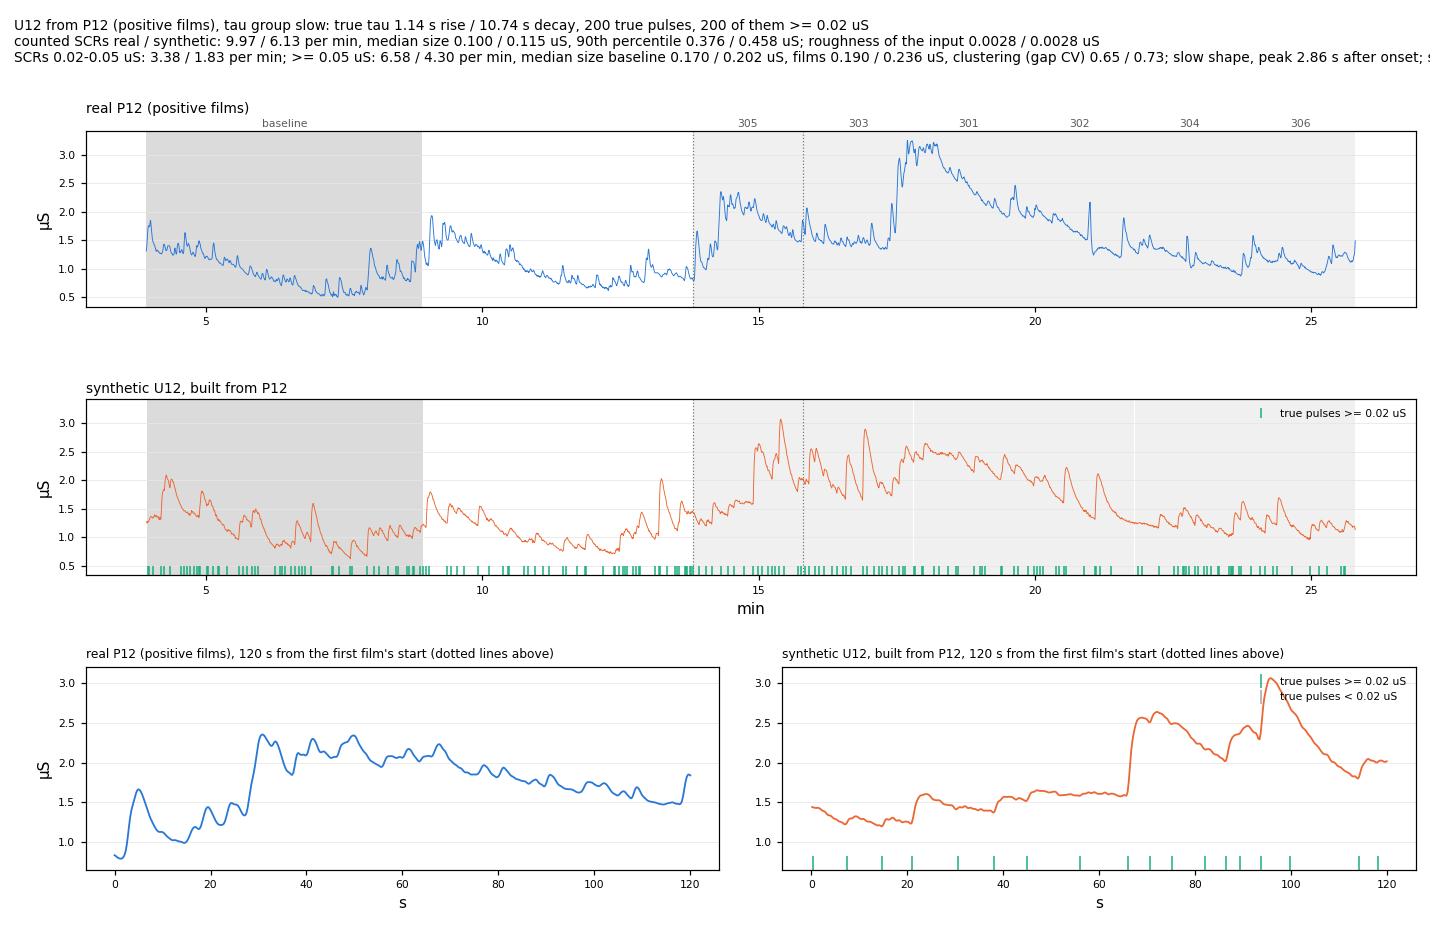
\includegraphics[width=0.92\textwidth,trim={0 0 0 52bp},clip]{figures/synth_vs_real_U12.png}
\caption{A real participant (P12, top) and the synthetic tuning session built from them (U12,
middle; true pulses of at least 0.02\uS{} marked), and 120\,s from the first film's start of
each (bottom). The session keeps the participant's timeline, tonic, response rates and sizes and
noise, with a randomly drawn slow response shape. Shading: baseline (dark) and films (light).}
\label{fig:synth}
\end{figure*}

\subsection{Tuning and Evaluation}\label{sec:tuning}
Settings were tuned on known truth only, never on fit alone, since a near-perfect fit can hide a
wrong response shape. Each round changed one setting; from round~7 on, the rule for accepting a
change was stated before the run. Rounds 1--5 used an earlier generator; rounds 6--8 used the U
sessions. The frozen setting was then evaluated once on the V sessions and run on the 50 real
participants.

Estimated and true impulses are matched one to one, closest pairs first, within 1\,s. Recall is
over true impulses of at least 0.02\uS{} (the smallest response peak detection can see),
precision over all returned impulses, and F1 combines them. The same scores are computed for the
stronger pulses: recall over true impulses of at least 0.05\uS{} matched against all returned
ones, and precision over returned impulses of at least 0.05\uS{} matched against all true ones.
Timing error, the rank correlation of matched sizes, and the error of the median $\tau$ over
windows complete the scores.

The re-synthesis test rebuilds each real signal from our own deconvolution of it and adds white
noise at the participant's own fit residual (median SD 0.0144\uS, about 25\,dB below the phasic
part), following the method of \cite{amin2021}; the result is deconvolved again and scored
against our own pulses. Without truth on the real recordings, we check the fit, count the pulses
returned under each isolated SCR (no other peak of at least 0.02\uS{} from 5\,s before its onset
to its half-recovery) and compare with the same count on the V sessions, correlate each
participant's pulse rate with their counted response rate, and compare with other deconvolution
methods run on the same dataset.

\subsection{Stage 2: Arousal State Estimation}\label{sec:stage2}
\todo{To be completed: the state-space model linking the pulse train to a continuous arousal
state, its estimation, and the statistical tests of H1--H6.} Two rules were fixed before H1--H6
were examined: the main analysis uses pulses of at least 0.05\uS{} (test F1 0.96), with all
pulses of at least 0.02\uS{} (F1 0.82) as the secondary check; and films are compared with each
participant's own baseline.

%=====================================================================
\section{Results}\label{sec:results}

\subsection{Sequence of Experiments}
Each round answered a question raised by the one before it (Table~\ref{tab:rounds}). Round~1
varied the two settings the published solver had kept fixed, the prior's weight $\lambda_3$ and the knot
spacing: knots every 14\,s kept the tonic from absorbing slow responses, but every setting found
only about half of the pulses. The cause was in the code: FOCUSS+ never restores a zeroed impulse,
so phase~1 bounds what phase~2 can find, and the phase-1 cap $\lambda_{\max}$ on the sparsity
weight $\lambda_2$, which the paper does not state, was too strict. Lowering it tenfold (round~2) recovered the missing pulses; lowering it
further admitted false ones. The fitted rises then showed a floor near 0.6\,s, consistent with the
0.5\,Hz filter smearing each response, which the new input of Section~\ref{sec:prep} removed
(round~3). The decays, however, were still pulled toward the prior's mean, so round~4 weakened the
prior to 1000 times below the paper's weight; removing it entirely made the fits unstable.
Round~5 confirmed that the knot spacing did not explain the remaining decay errors.

The setting frozen after round~5 kept its accuracy on test sessions from the early generator, but
on real data the $\lambda_2$ chosen by GCV sat at its cap in most windows (91\%, against 38\% in
tuning): the synthetic signals were not on the real signals' scale, so settings tuned on them could
not be defended. This motivated the participant-matched generator (Section~\ref{sec:synth}) and
round~6 on its sessions, which asked whether scale should be controlled. Normalizing each session
lowered accuracy, since the noise is roughly constant in $\mu$S and scaling small responders up
amplifies it; halving or doubling the input only traded recall against precision; and raising
GCV's cap on $\lambda_2$ tenfold changed nothing. The solver therefore runs in $\mu$S with the paper's 8 random starts,
and was frozen and evaluated once (Section~\ref{sec:test}). Rounds~7 and~8 then asked whether the
prior or the tonic causes the remaining errors on slow responses (Section~\ref{sec:errors}).

\begin{table*}[t]
\centering
\caption{Tuning Rounds: Change, Result and Decision (Median F1 Over the 18 Tuning Sessions)}
\label{tab:rounds}
\footnotesize
\setlength{\tabcolsep}{4pt}\begin{tabular}{@{}cp{5.0cm}p{6.4cm}p{4.6cm}@{}}
\toprule
Round & Change & Result & Decision \\
\midrule
1 & Prior weight $\lambda_3$ (3 levels) $\times$ knots (6, 14\,s) & 14\,s best (F1 0.60 vs 0.47); recall only 0.41 & Knots 14\,s; find the missing pulses \\
2 & Phase-1 cap $\lambda_{\max}$ on $\lambda_2$: $10^{-2}\to10^{-3}$, $10^{-4}$ & F1 0.58 $\to$ 0.81; at $10^{-4}$ precision 0.74 & $\lambda_{\max}=10^{-3}$ ($2\cdot10^{-3}$ at 4\,Hz) \\
3 & Input 0.5\,Hz / 2\,Hz $\to$ 1\,Hz / 4\,Hz & F1 0.81 $\to$ 0.85; rise floor 0.6 $\to$ 0.5\,s & 1\,Hz / 4\,Hz input \\
4 & $\lambda_3$ 10$\times$ lower; no prior ($\lambda_3=0$) & F1 0.84; slowest-shape decay error $-23\% \to -4\%$; no prior unstable & $\lambda_3=10^{-4}$ ($2\cdot10^{-4}$ at 4\,Hz) \\
5 & Knots 10, 20\,s & No difference (F1 0.89--0.90) & 14\,s; frozen for the first real run \\
\midrule
6 & Normalization; input $\times0.5$, $\times2$; GCV cap on $\lambda_2$ $\times10$; 8 starts & 0.835 (normalized 0.792; $\times0.5$ 0.815; $\times2$ 0.784; cap 0.827) & $\mu$S, 8 starts; frozen \\
7 & No prior ($\lambda_3=0$) & 0.825; fewer windows meet the selection rule & Weak prior kept \\
8 & Knots 20, 28\,s & 0.803, 0.794; more false pulses & 14\,s kept \\
\bottomrule
\multicolumn{4}{@{}p{16.9cm}@{}}{\scriptsize Rounds 1--5 on the earlier generator's sessions, 6--8 on the
participant-matched U sessions; rounds 1--4 report F1 over all pulses, 5--8 over pulses of at
least 0.02\uS.}
\end{tabular}
\end{table*}

\subsection{Unseen Test Sessions}\label{sec:test}
On the 50 V sessions the frozen solver recovers pulses of at least 0.05\uS{} with F1 0.96, recall
0.98 and precision 0.96, and all pulses with F1 0.82 (Table~\ref{tab:test}, Fig.~\ref{fig:test}).
The errors concentrate at the noise floor: on the tuning sessions, 92\% of missed and 80\% of
false pulses were below 0.05\uS. Accuracy is the same in every film group, so it cannot by itself
produce a group difference in H1--H4. Timing is within 0.16\,s and the rank correlation of sizes
is 0.98. The time constants come out with median errors of $+9\%$ (rise) and $-13\%$ (decay);
slow responses are the hard case, with decays 37\% short and precision 0.75 over all pulses.

\begin{table}[t]
\centering
\caption{Accuracy on Synthetic Data (Medians)}
\label{tab:test}
\footnotesize
\setlength{\tabcolsep}{3pt}
\begin{tabular}{@{}lcccc@{}}
\toprule
 & \multicolumn{2}{c}{Test, 50 unseen} & \multicolumn{2}{c}{Re-synthesis, 50} \\
\cmidrule(lr){2-3}\cmidrule(l){4-5}
 & $\ge$0.05\uS & all & $\ge$0.05\uS & all \\
\midrule
F1 & \textbf{0.96} & 0.82 & 0.96 & 0.86 \\
Recall & 0.98 & 0.85 & 0.95 & 0.89 \\
Precision & 0.96 & 0.85 & 0.97 & 0.84 \\
F1, fast shapes & 0.98 & 0.83 & -- & -- \\
F1, typical shapes & 0.97 & 0.84 & -- & -- \\
F1, slow shapes & 0.94 & 0.79 & -- & -- \\
F1, film groups & 0.95--0.97 & 0.80--0.83 & 0.93--0.96 & 0.84--0.88 \\
Timing error & \multicolumn{2}{c}{0.16\,s} & \multicolumn{2}{c}{0.15\,s} \\
Size rank corr. & \multicolumn{2}{c}{0.98} & \multicolumn{2}{c}{0.92} \\
Rise error & \multicolumn{2}{c}{$+9\%$} & \multicolumn{2}{c}{$-14\%$} \\
Decay error & \multicolumn{2}{c}{$-13\%$} & \multicolumn{2}{c}{$+26\%$} \\
\bottomrule
\end{tabular}
\end{table}

\begin{figure*}[t]
\centering
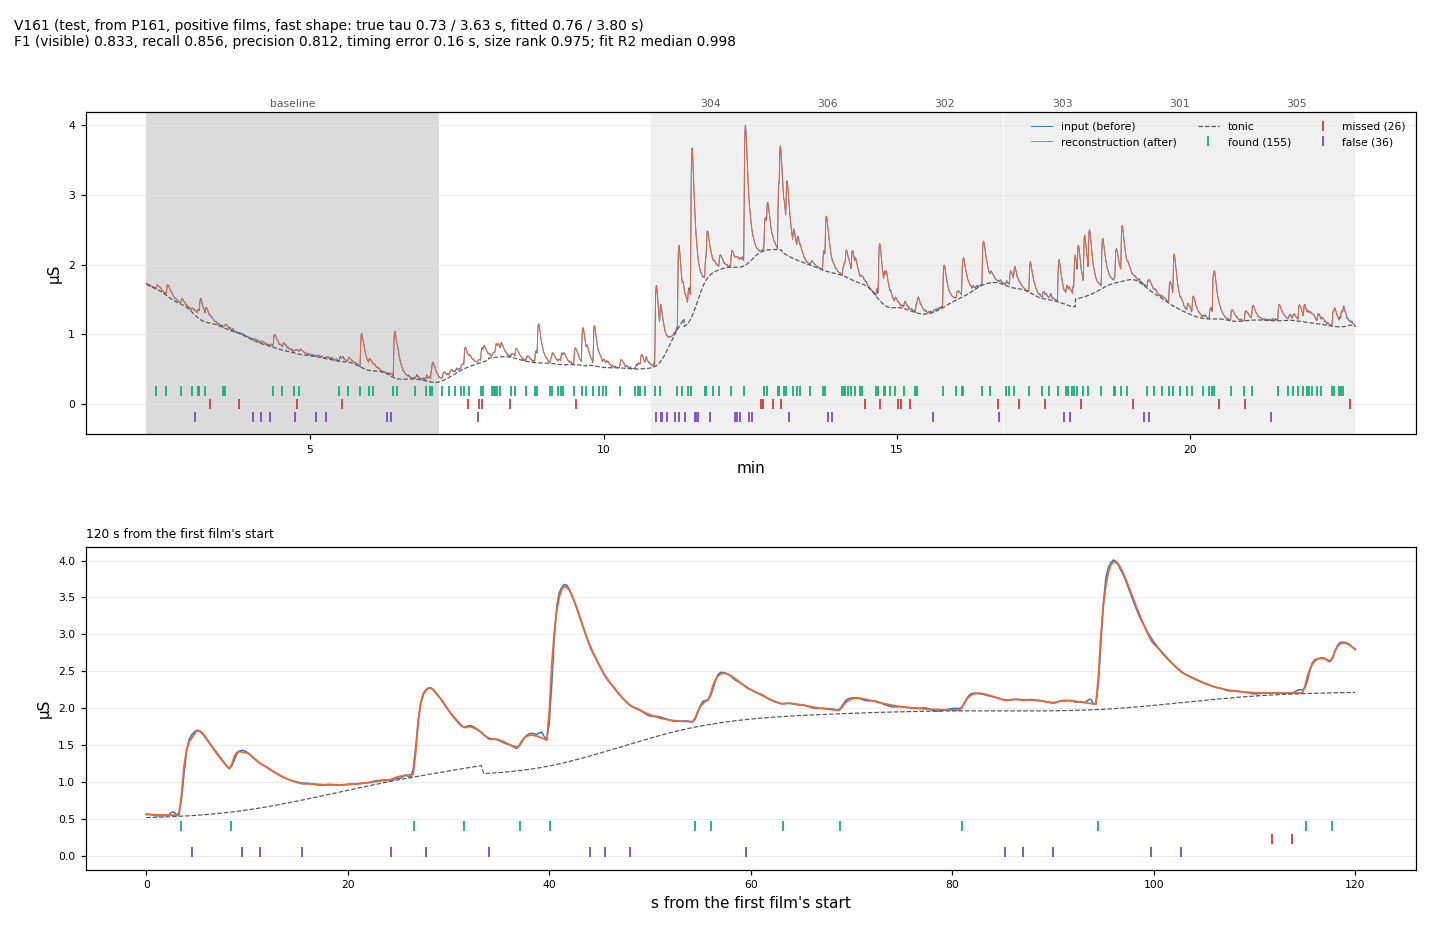
\includegraphics[width=0.92\textwidth,trim={0 0 0 56bp},clip]{figures/test_V161.png}
\caption{Deconvolution of an unseen test session (V161, fast response shape): input, reconstruction
and estimated tonic, with found (green), missed (red) and false (purple) pulses, over the whole
session (top) and 120\,s from the first film's start (bottom). F1 over all pulses 0.83, close to the
test median.}
\label{fig:test}
\end{figure*}

\subsection{Re-synthesis}
Rebuilt from its own output, the solver recovers its pulses with F1 0.96 at 0.05\uS{} and 0.86
over all pulses, again equally in every film group (Table~\ref{tab:test}). The test is circular,
so it measures self-consistency under realistic noise, not accuracy. It adds one finding: rebuilt
from its own time constants, the solver returns decays 26\% longer.

\subsection{Remaining Errors: Prior and Tonic}\label{sec:errors}
Removing the prior (round~7) did not improve accuracy and made the fits less stable, most of all
on slow shapes, where far fewer windows met the selection rule. A prior measured directly on the
real waveforms, without any model, failed the accuracy check we set for it on the test sessions
and was not used. The prior's mean and standard deviation are therefore those of
\cite{amin2021}; refitting them to our own estimates would feed the solver's biased output back
into it.

The tonic's flexibility is set by its knots alone: GCV leaves $\lambda_1$ near zero, because the
penalty acts on the spline coefficients, which encode the tonic's level rather than its shape.
Wider knots (round~8) missed fewer small pulses but returned many more false ones, where the real
tonic changes faster than a stiffer spline can follow. During dense slow responding the estimated
tonic sits above the true one at every knot spacing, by 0.2--0.4\uS{} (Fig.~\ref{fig:tonic}):
overlapping long recoveries never let the signal return to its floor, so the data hold no
information about it, and a higher tonic with shorter decays fits about as well. This is why slow
decays come out short with or without the prior. On fast and typical shapes the bias is reversed:
the test sessions, the re-synthesis and a direct measurement on the real waveforms all show
decays that are too long.

\begin{figure*}[t]
\centering
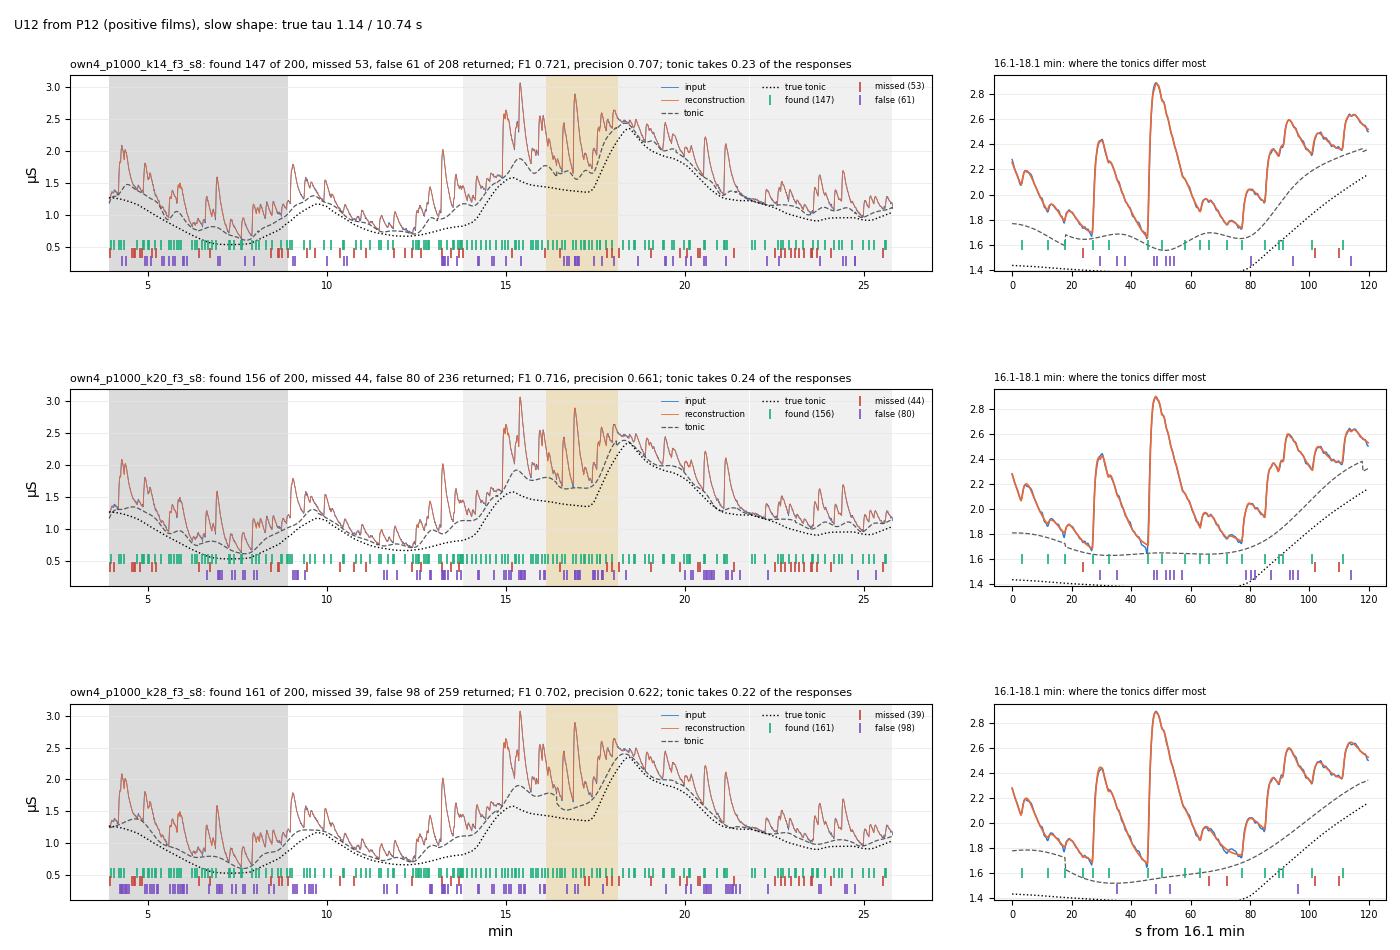
\includegraphics[width=0.92\textwidth,trim={0 0 0 33bp},clip]{figures/tonic_round8_U12.png}
\caption{The same slow tuning session (U12) deconvolved with knots every 14\,s (frozen setting,
top), 20\,s and 28\,s, whole session (left) and the 120\,s where the estimated tonics differ most
(right). Dashed: estimated tonic; dotted: true tonic. At every spacing the estimated tonic sits
above the true one during dense slow responding.}
\label{fig:tonic}
\end{figure*}

\subsection{Real Participants}
On the 50 real recordings the reconstruction fits closely (median $R^2=0.999$;
Fig.~\ref{fig:real}), and the solver returns about twice as many pulses as there are counted
responses (11.7 against about 7 per minute). Two effects explain this. First, counting merges
overlapping responses into one: on synthetic data it finds only about three in four true pulses,
while deconvolution separates them. Second, the solver adds a small excess on real data: under
isolated responses, where the two can be compared directly, it returns as many pulses as are true
on the test sessions but about 16\% more on the real recordings (Table~\ref{tab:isolated}),
mostly small pulses placed 1--2\,s apart on response rises rather than in quiet stretches.
Sparser settings do not remove these selectively: in rounds~2 and~6 they lost true pulses at
least as fast as false ones.

The pulse counts are consistent with independent evidence. Each participant's pulse rate tracks
their own counted response rate (rank correlation 0.73), and the published solver \cite{amin2021}
and cvxEDA \cite{greco2016} return comparable rates on the same dataset. No reference range exists
for deconvolved pulses, since published norms count visible responses: about 1--3 per minute at
rest at 0.05\uS{} (Dawson et al., as cited in \cite{kurinec2022}) and up to about 10 at lower
thresholds (Zimmer, as cited in \cite{gertler2020}). Our participants already show 4.6 counted
responses of at least 0.05\uS{} per minute at rest, an active sample consistent with selection on
response size.

\begin{table}[t]
\centering
\caption{Pulses Returned Under Each Isolated SCR (Mean)}
\label{tab:isolated}
\footnotesize
\setlength{\tabcolsep}{4pt}
\begin{tabular}{@{}lccc@{}}
\toprule
 & Test: true & Test: returned & Real: returned \\
\midrule
On the rise, all & 1.23 & 1.24 & \textbf{1.44} \\
On the rise, $\ge$0.05\uS & 1.13 & 1.18 & 1.27 \\
On the recovery, all & 0.17 & 0.33 & 0.31 \\
Rises with 1 / 2 / 3+ pulses & 79 / 19 / 2\% & 78 / 20 / 2\% & 62 / 26 / 10\% \\
\bottomrule
\multicolumn{4}{@{}p{8.2cm}@{}}{\scriptsize 452 isolated SCRs on the 50 test sessions, 444 on the
50 real recordings. Rise: from 1\,s before onset to the peak; recovery: from the peak to
half-recovery.}
\end{tabular}
\end{table}

\begin{figure*}[t]
\centering
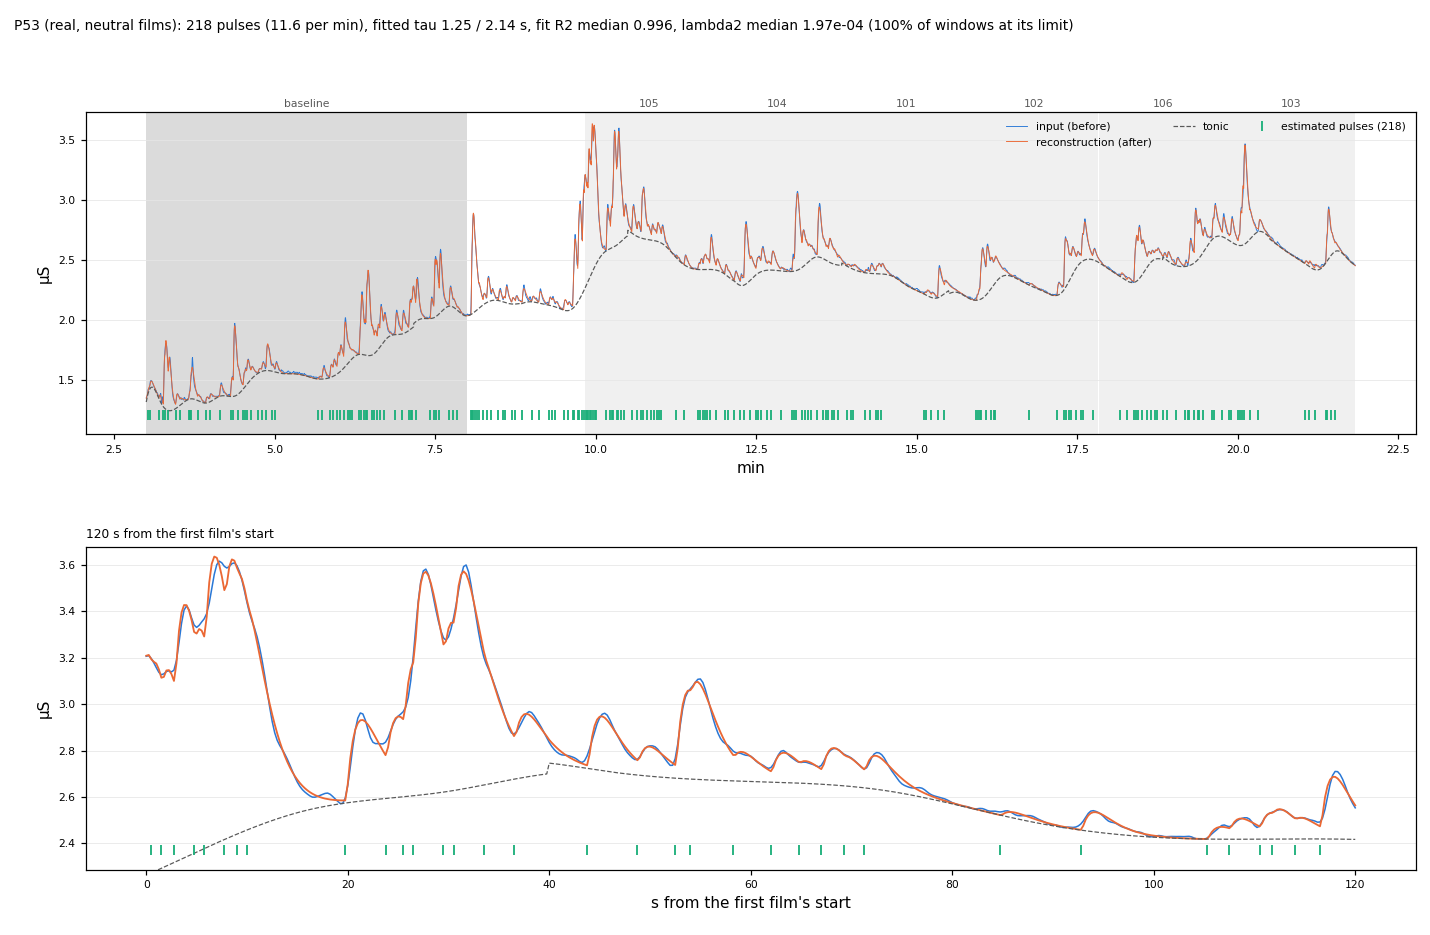
\includegraphics[width=0.92\textwidth,trim={0 0 0 56bp},clip]{figures/real_P53.png}
\caption{Deconvolution of a real participant (P53, neutral films): input, reconstruction and
estimated tonic with the estimated pulses, over the whole session (top) and 120\,s from the first
film's start (bottom).}
\label{fig:real}
\end{figure*}

\subsection{Arousal State and Hypotheses}
\todo{Stage 2 results: the estimated arousal state of each participant, and the tests of H1--H6.}

Before stage 2, one descriptive look at the pulses by block was taken after the solver, the
selection and the 0.05\uS{} threshold were frozen, without tests (Table~\ref{tab:blocks}).
Relative to each participant's own baseline, the groups shown emotional films kept or raised their
responding, while the neutral group's fell. Film rates were not above baseline in most groups;
the baseline comes first and responding usually fades over a session, which is why stage 2
compares films with each participant's own baseline. Pulse size was added to this look after the
rates had been seen.

\begin{table}[t]
\centering
\caption{Descriptive Look: Films Relative to Each Participant's Baseline (Median Ratio, Pulses
$\ge$0.05\uS, No Tests)}
\label{tab:blocks}
\footnotesize
\begin{tabular}{@{}lcccc@{}}
\toprule
Group ($n$) & Rate & Size & Rate $\times$ size & Films \\
\midrule
Neutral (20) & 0.77 & 1.01 & 0.81 & neutral \\
Negative (10) & 0.93 & 1.16 & 1.14 & negative \\
Positive (10) & 1.01 & 0.99 & 1.01 & positive \\
Mixed (10) & 1.21 & 1.09 & 1.34 & negative, positive \\
\bottomrule
\end{tabular}
\end{table}

%=====================================================================
\section{Discussion}

Where the truth is known, the solver recovers pulses of at least 0.05\uS{} almost completely
(recall 0.98) and almost only real ones (precision 0.96), on synthetic sessions built from the
same participants it is applied to. On the real recordings its behaviour matches that, apart from
a small excess of doublets, and its pulse rates agree with each participant's visible responding
and with other deconvolution methods on the same data. Pulses of 0.02--0.05\uS{} are recovered
less reliably, which is why stage 2 uses the stronger pulses as its main input.

The limitations to keep in mind are:
\begin{itemize}
\item Slow responses (half-recovery above 7\,s): decays 37\% short and lower precision, because
the true tonic level is never visible during dense slow responding; neither the prior nor the
knot spacing changes it.
\item On fast and typical shapes the decays run long, so the real decays (median 3.4\,s) are
likely overestimated.
\item False pulses appear where the tonic rises faster than its knots allow.
\item About 8--20\% extra small pulses on response rises in the real data, about half of them
below 0.05\uS; 36\% of isolated real SCRs recover as fast as they rise, a shape the model cannot
produce.
\item The generator does not time responses to specific moments, merges large responses twice,
and uses the same response model as the solver, which favours model-based methods in any
comparison on these data.
\item The sparsity exponent $p=0.5$ comes from earlier code \cite{faghih2014} and was not tuned.
\end{itemize}

A comparison with cvxEDA \cite{greco2016} and the published solver under identical conditions on
the V sessions is the natural next test of the method choice; it would also test a different
treatment of the tonic without circularity. \todo{Discussion of the stage-2 results and the
hypotheses.}

%=====================================================================
\section{Conclusion}

An open re-implementation of the sparse deconvolution of \cite{amin2021}, tuned on synthetic
sessions that copy each participant, recovers sudomotor pulses of at least 0.05\uS{} with F1 0.96
on unseen sessions and behaves consistently on the real recordings of 50 participants watching
emotional films. Its remaining errors are confined to small pulses and to slow, densely
overlapping responses, where the tonic cannot be separated from the phasic part.
\todo{Conclusion on the arousal state and H1--H6.}

\bibliographystyle{IEEEtran}
\bibliography{refs}

\end{document}
